\documentclass{beamer}
\usepackage[utf8]{inputenc}
\usepackage{listings}
\usepackage{svg}

\usetheme{Madrid}
\definecolor{sigaipurple}{rgb}{0.30, 0.16, 0.44}
\setbeamertemplate{caption}{\raggedright\insertcaption\par}

\useoutertheme{infolines} % Alternatively: miniframes, infolines, split
\useinnertheme{circles}
\usecolortheme[named=sigaipurple]{structure}

\lstset{basicstyle=\footnotesize\ttfamily,breaklines=true}

%------------------------------------------------------------
%This block of code defines the information to appear in the
%Title page
\title[Python \& Numpy] %optional
{Python Fundamentals \& Numpy}

\subtitle{"Back to square \textit{zero}"}

\author[SIGAI] % optional
{A.~Shen, A.~Singh, S.~Sharief} 

\date{September 12, 2022}

\titlegraphic{
\includegraphics[width=5cm]{../shared/logo.png}}

%End of title page configuration block
%------------------------------------------------------------



%------------------------------------------------------------
%The next block of commands puts the table of contents at the 
%beginning of each section and highlights the current section:

\AtBeginSection[]
{
  \begin{frame}
    \frametitle{Table of Contents}
    \tableofcontents[currentsection]
  \end{frame}
}
% ------------------------------------------------------------


\begin{document}

%The next statement creates the title page.
\frame{\titlepage}


%---------------------------------------------------------
% This block of code is for the table of contents after
% the title page
\begin{frame}
\frametitle{Table of Contents}
\tableofcontents
\end{frame}
%---------------------------------------------------------


\section{Why it's Worth Your Time}
%---------------------------------------------------------
%Changing visibility of the text

\begin{frame}{Let's Talk Python}
	\begin{center}
		Python is interpreted\pause, high-level\pause, dynamically typed \pause \& garbage collected. \newline \\ \pause
	\end{center}

	\begin{center}
		Pretty awesome, yeah?
	\end{center}
\end{frame}

\begin{frame}{Why Numpy}
	Well, it's \textit{very} slow. 
	\begin{figure}[h!]
		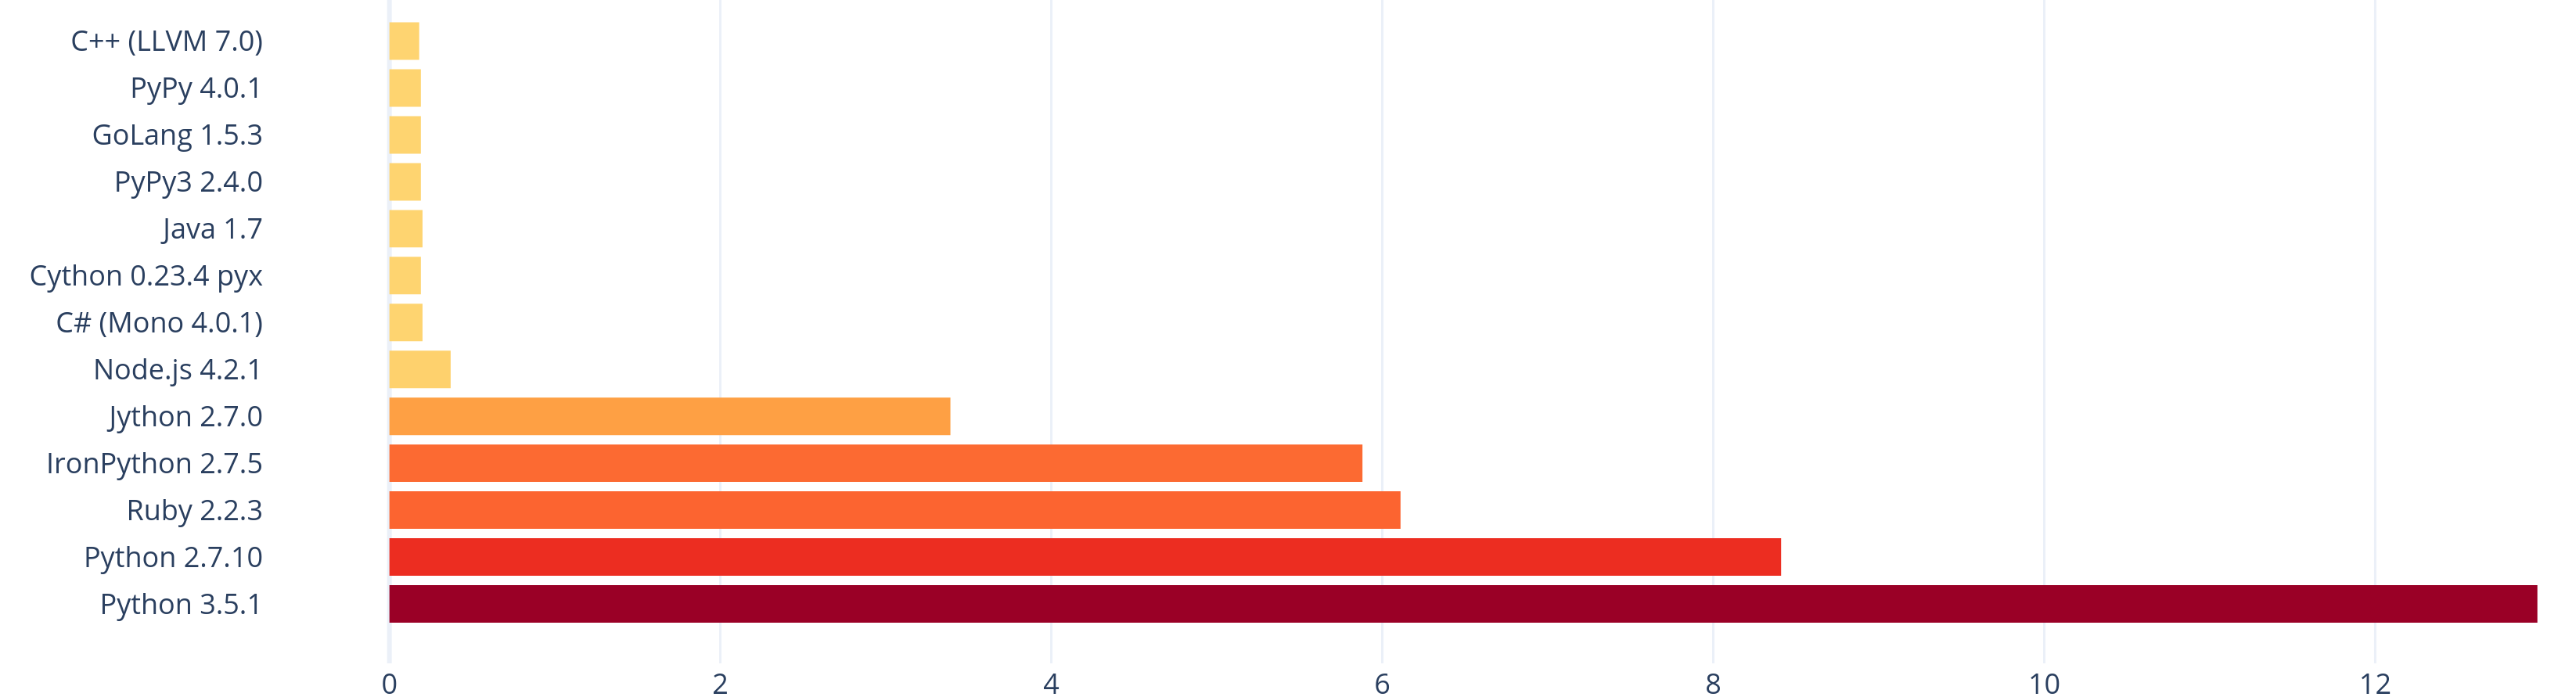
\includegraphics[width=0.9\textwidth]{images/speed}
		\caption{\href{https://www.snazar.com/articles/how-slow-is-python/}{Time(s) to complete BuildBridge with D=9, L=1}} % from "How Slow Is Python?" by Sam Nazarian
	\end{figure} \pause
	If we want to brew millions of parameters worth of linear algebra soup, we need \textbf{speed}. \newline \\ \pause
	Python is very easy to work with. C, C++ are fast but unintuitive. 
\end{frame}

\begin{frame}{Why Numpy}
	Can't be too hard to guess a solution? \newline \\ \pause 
	Enter \href{https://numpy.org/}{NumPy}:
	\begin{center}
		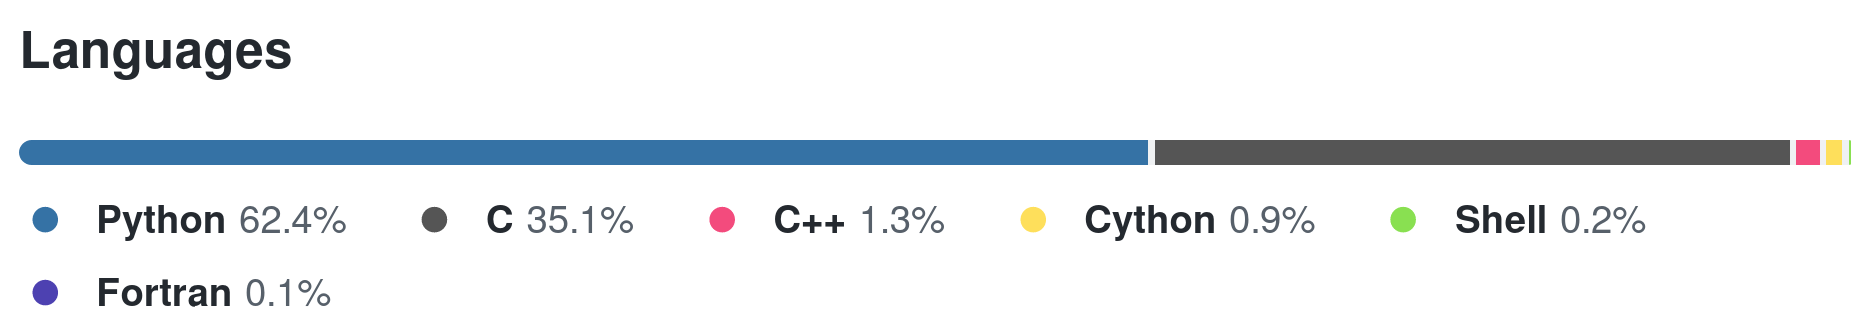
\includegraphics[width=0.8\textwidth]{images/np-langsplit}
	\end{center} \pause
	By effectively using Python as a \textit{wrapper}, we delegate compute-intensive tasks to LLVM infrastructure, while maintining ease-of-use. \newline \\
	\textit{Voilà}; best of both worlds.
\end{frame}

\section{Bootsrapping Terminology}

\begin{frame}{Categorizing Popular Learning Methods}
\end{frame}

\section{Python for ML}

\section{Nailing Numpy}

\begin{frame}{Thank you!}
	\begin{center}
		Have an awesome rest of your day!
	\end{center}
	\begin{center}
		\textbf{Slides:} \texttt{\url{https://cs.purdue.edu/homes/jsetpal/slides/python-numpy.pdf}}
	\end{center}
\end{frame}

\end{document}
